\section{Server Configuration for Distributed Resolver Agents}\label{sec:resolver-server}

Implementing the distributed resolver agents requires an AMQP message queue server that
is used for communication between the \cxoneflow server and the distributed resolver
agents.  Details about the message queue deployment can be found in Section \ref{sec:external-mq}.

The examples in this section show a configuration that uses team names as tags to establish
build environment affinity to \scaresolver scanning.  The tags can be used to establish
the build environment affinity in whatever way fits your organization best.

\subsection{\cxoneflowtext\space Endpoint Configuration}

The endpoint server \intlink{sec:yaml-config}{YAML configuration} will not utilize resolver agents
by default.  Using resolver agents requires a public/private key pair; the private key is configured
for use on the \cxoneflow endpoint and the public key is distributed with each resolver agent.  Before
configuring the use of distributed resolver agents, it is recommended to read about the security
concepts in Section \ref{sec:resolver-agent-security}.

The \cxoneflow endpoint will send messages signed by the private key to the distributed resolver
agents using the message queue.  The distributed resolver agents will validate the signature
using the public key; if the signature is not valid, the resolver agents will reject the message.

Distributed agents are identified using agent tags.  The \cxoneflow endpoint is configured by the
administrator with a list of allowed tags to prevent arbitrary agents from appearing.  The
server-side tag configuration is also used to set up the communication with the agents via
the message queue.  Anyone who installs a resolver agent must configure it to respond to messages
targeting at least one valid agent tag.


\subsubsection{Generating a Public/Private Key Pair}\label{ref:server-key-pair}

There are many ways to generate a public/private key pair.  There are only a few requirements
for key pairs produced by any method:

\begin{itemize}
  \item The private key must be unencrypted.
  \item Both the private and public key files must be PEM encoded.
  \item The public/private key algorithm is supported by the install Python \texttt{cryptography} library.
    As of this release, these algorithms have been tested:
  \begin{itemize}
      \item RSA 4096-bit
      \item ECDSA secp256k1
  \end{itemize}
\end{itemize}

One easy method of generating a public/private key pair is to use OpenSSL.  To generate an ECDSA public/private key pair,
the following command can be used.  The command will create the file \texttt{ec-priv.pem} that holds the unencrypted private key
and the file \texttt{ec-pub.pem} that holds the public key.

\begin{code}{OpenSSL Public/Private Key Creation}{[ECDSA]}{}
openssl ecparam -name secp256k1 -genkey -noout | tee ec-priv.pem | openssl ec -pubout > ec-pub.pem  
\end{code}

To generate an RSA 4096-bit public/private key pair,
the following command can be used.  The command will create the file \texttt{rsa-priv.pem} that holds the unencrypted private key
and the file \texttt{rsa-pub.pem} that holds the public key.

\begin{code}{OpenSSL Public/Private Key Creation}{[RSA]}{}
openssl genrsa 4096 |tee rsa-priv.pem | openssl rsa -pubout > rsa-pub.pem
\end{code}

The private key file may be stored as a secret referenced in the configuration YAML element \intlink{sec:yaml-resolver-private-key}{resolver->private-key}.

\subsubsection{Resolver YAML Configuration}\label{sec:resolver-yaml-config}
Figure \ref{fig:resolver-config-yaml} shows the common YAML configuration for resolver agents with a list of allowed tags.
This YAML configuration is provided in the configuration example artifacts that can be downloaded from the \cxoneflow release
artifacts.

Some of the things to note in these examples:

\begin{itemize}
  \item The AMQP URL is stored as a secret since it contains credentials.
  \item The AMQP connection is common in both the \texttt{feedback} and \texttt{resolver} configuration.
  This configuration allows the feedback workflows and resolver workflows to use the same external message queue.
  \item The resolver configuration is often easily maintained as a common configuration that is applied to 
  all service definitions for all SCM types.  
\end{itemize}


\begin{figure}[h]
    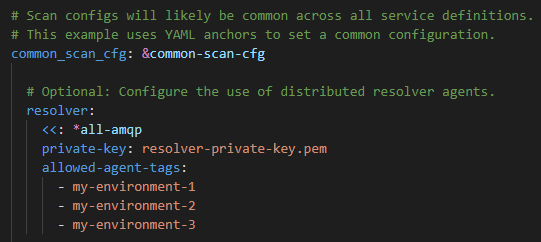
\includegraphics[width=\textwidth]{graphics/resolver-config-yaml.png}
    \caption{Resolver Common Configuration for Server YAML}
    \label{fig:resolver-config-yaml}
\end{figure}


\subsection{Message Queue Configuration}

The \cxoneflow endpoint will configure the AMQP Exchanges and Queues upon start.  Adding any
allowed agent tags will require at least one \cxoneflow endpoint restart so that the
appropriate message queue elements for that tag can be constructed.

The message queue connection credentials for the \cxoneflow endpoint will have the 
permissions required to enable configuring the message queue elements.  Section \ref{sec:external-mq}
will give more details about the appropriate message queue user permissions for the \cxoneflow endpoint.

Configuring a distributed resolver agent will require each agent to have credentials that allow limited
access to the message queue.  Section \ref{sec:resolver-agent-security} has more details about the
authorization that should be assigned to credentials used by distributed agents.

The YAML examples in \intlink{sec:resolver-yaml-config}{the previous section} demonstrated the use of a single
message queue instance for both the communication with the distributed resolver agents and feedback workflow
orchestration.  While using a single message queue may make the \cxoneflow configuration simpler, it is not
strictly required to use the same message queue connection for all configurations.  Each configuration can
use a segregated message queue server if this is desired.  This segregation includes the use
of \extlink{https://www.rabbitmq.com/docs/vhosts}{virtual hosts} if supported by the AMQP endpoint server.


\subsection{Deployment Considerations}

The YAML examples in \intlink{sec:resolver-yaml-config}{the previous section} demonstrated agent tags
configured in a single endpoint service definition.  The allowed tags in each service endpoint are
indicating which agent tags can perform resolver scans for an event handled by that service endpoint.
The tags are used to communicate with agents that listen for messages directed to that agent tag and
have the public key associated with the private key defined in the service configuration.

The important thing to note is that distributed resolver agents are not tied to a single
\cxoneflow endpoint service definition.  The distributed resolver agents will typically have
tooling and configuration that can be used for any code that requires that tooling.  This
has some implications in how distributed resolver agents can be deployed:

\begin{itemize}
  \item One instance of a distributed resolver agent can handle multiple tags.
  
  \item More than one instance of a distributed resolver agent can be deployed to handle the same tag.

  \item The distributed resolver agent tag/private key pair can be different in each service definition.  It is recommended to
  use duplicate distributed resolver agent tags across \cxoneflow service definitions only when those tags all share the same public/private
  key pair.

  \item Not all service definitions need to support the same allowed agent tags.  If there are distributed agents
  that should only be used by a specific service definition, it is recommended to use the allowed agent tag list
  in combination with distributed resolver connection credentials that limit the agent's ability to receive
  communications for specific tags.

  \item For complex \cxoneflow configurations that have many service definitions, it is recommended to engineer
  deployment of distributed resolver agents to be as simple as possible.
    
\end{itemize}


